\documentclass[a4paper]{article}

\usepackage[francais]{babel}
\usepackage[latin1]{inputenc}
\usepackage[T1]{fontenc}
%\usepackage{amsmath}
\usepackage{graphicx}
\usepackage[colorinlistoftodos]{todonotes}
\usepackage{comment}
\usepackage{float}
\usepackage[colorlinks=true,linkcolor=black,citecolor=black]{hyperref}

\title{\bsc{INSA} de Rennes \\ D\'epartement Informatique \\ \bigskip \hrule \bigskip Syst\`eme d'annotation et de navigation dans des images d'archives \\ \bigskip Rapport de pr\'e-\'etude \bigskip \hrule}
\author{Rapha\"el \bsc{Baron}, Pierre-Olivier \bsc{Bouteau}, Nicolas \bsc{Charpentier}, \\ Cl\'ement \bsc{Leboullenger}, Thomas \bsc{Fran\c{c}ois}, Benoit \bsc{Travers}}

\begin{document}
\maketitle
\thispagestyle{empty}
\newpage

\tableofcontents
\thispagestyle{empty}
\newpage

\section{Introduction}

	Les Archives d\'epartementales d'Ille-et-Vilaine sont en charge de la collecte, du classement, de la conservation et de la communication des archives qui constituent une grande partie du patrimoine historique \'ecrit du d\'epartement \cite{archive35}. 
\`A l'approche du centenaire de la Premi\`ere Guerre Mondiale, les Archives, en collaboration avec l'\bsc{INSA} de Rennes, ont choisi de proposer aux \'etudiants en quatri\`eme ann\'ee du d\'epartement informatique un sujet de mise en valeur des documents li\'es \`a la Grande Guerre.

	L'objectif du projet sera de construire un outil d'annotations semi-auto\-matique des documents li\'es au recrutement militaire concernant cette p\'eriode. L'outil devra permettre \`a un utilisateur, visiteur des archives, d'associer lecture et annotation du document avec l'image num\'eris\'ee qui lui correspond. En plus de naviguer et d'annoter les images, l'usager pourra utiliser ces annotations pour rechercher des documents, par exemple trouver une personne gr\^ace a son nom.
\\

	Ce rapport de pr\'e-\'etude introduit le contexte et les donn\'ees essentielles \`a la compr\'ehension du besoin \`a l'origine du projet, avant de sp\'ecifier ce m\^eme besoin. 
La m\'ethodologie de gestion de projet, une premi\`ere planification et les partenaires qui contribuent \`a la r\'ealisation du projet sont aussi pr\'esent\'es.

	Le projet sera encadr\'e par Mme Marie \bsc{Babel}, ma\^itre de conf\'erences \`a l'\bsc{INSA} de Rennes et M. Ivan \bsc{Leplumey}, directeur du d\'epartement informatique de l'\bsc{INSA} de Rennes. 
Mme Karen \bsc{F\'evrier}, chef de projet chez \bsc{ATOS} sera \'egalement sollicit\'ee sur les aspects de gestion de projet. 
Un contact r\'egulier avec M. Jean-Yves \bsc{Le Clerc}, adjoint au directeur des Archives d\'epartementales d'Ille-et-Vilaine permettra enfin de cibler au mieux le projet sur les besoins des Archives.
\\

	Il sera r\'ealis\'e par MM. Rapha\"el \bsc{Baron}, Pierre-Olivier \bsc{Bouteau}, Nicolas \bsc{Charpentier}, Cl\'ement \bsc{Leboullenger}, Thomas \bsc{Fran\c{c}ois} et Benoit \bsc{Tra\-vers}, \'etudiants en quatri\`eme ann\'ee au d\'epartement informatique de l'\bsc{INSA} de Rennes.

\newpage

\section{Contexte et sujet}
\label{sec:contexte}

\subsection{Un client : les Archives d\'epartementales d'Ille-et-Vilaine}
\label{subsec:client}

	Les Archives d\'epartementales ont \'et\'e cr\'e\'ees dans chaque d\'epartement en vertu de la loi du 5 brumaire an V (26 octobre 1796). Elles \'etaient destin\'ees \`a conserver les archives de l'Ancien R\'egime (y compris celles des \'ev\^ech\'es, abbayes, etc) ainsi que les archives des nouvelles institutions. 
Nous avons eu la chance de visiter les Archives d\'epartementales d'Ille-et-Vilaine. Au cours de cette visite, nous avons appris que les Archives respectent la r\`egle des quatre C : Collecter, Conserver, Classer et Communiquer.
\\

	La premi\`ere mission des Archives est de \textbf{collecter} des documents. Les Archives d\'epartementales ne pouvant tout archiver par manque d'espace, s\'electionnent les archives produites par les administrations et les \'etablissements publics qui m\'eritent d'\^etre conserv\'ees au regard de l'Histoire. 
Les Archives d\'epartementales accueillent \'egalement les archives priv\'ees provenant notamment des associations, des entreprises et des particuliers.

	Vient ensuite la \textbf{conservation}. Chaque service d'Archives d\'epartementales g\`ere des fonds de documents originaux qui se comptent en kilom\`etres lin\'eaires. Afin de conserver ces documents dans les meilleures conditions possibles, les Archives disposent de salles climatis\'ees avec contr\^ole de la temp\'erature et de l'hygrom\'etrie.
    
	Cependant, en plus de l'usure du temps, les manipulations r\'eguli\`eres condui\-sent \`a une d\'egradation suppl\'ementaire. Pour pallier ce probl\`eme, le service de restauration des documents d\'et\'erior\'es n'est pas suffisant. C'est pourquoi les archives ont lanc\'e une politique de pr\'evention des risques de d\'egradation qui guide l'action des archivistes et des restaurateurs de documents. Les campagnes de microfilmage et de num\'erisation de documents fragilis\'es par le temps, ou tr\`es souvent consult\'es, garantissent leur transmission aux g\'en\'erations futures. Parmi les documents conserv\'es, figurent les registres paroissiaux Bapt\^emes-Mariages-S\'epultures (ancien r\'egime) (BMS) et Naissances-Mariages-D\'ec\`es (NMD), documents de base pour les g\'en\'ealogistes, qui constituent une partie importante des lecteurs fr\'equentant les archives.

	Cependant, collecter et conserver des documents sans aucune logique n'aurait pas de sens. C'est pour cela que les Archives \textbf{classent} tous les documents archiv\'es. Le personnel des Archives d\'epartementales effectue un rigoureux travail de tri et de classement pour \'elaborer des instruments de recherche (inventaires, r\'epertoires, fichiers, bases de donn\'ees...), outils indispensables pour orienter le lecteur.

	Enfin, afin de valoriser cette collection de documents, la \textbf{communication} est indispensable. Les Archives d\'epartementales mettent \`a disposition du public, en salle de lecture, les archives class\'ees. Les chercheurs et \'etudiants y trouvent les sources de leurs travaux historiques; les particuliers et les administrations des documents n\'ecessaires \`a l'\'etablissement de leurs droits.
Les g\'en\'ealogistes et les amateurs d'histoire locale y d\'ecouvrent leurs racines. Des expositions, des ateliers p\'edagogiques et des publications contribuent aussi \`a la mise en valeur du patrimoine du d\'epartement d'Ille-et-Vilaine. La communication passe aussi par une mise en ligne des documents d'archives. Cependant, la mise \`a disposition des documents en ligne entra\^ine une baisse des fr\'equentations des b\^atiments des Archives d\'epartementales.

    Afin de comm\'emorer le centenaire de la guerre 1914-1918, les Archives d'Ille-et-Vilaine ont pour projet de mettre en place, entre autres, un site permettant de consulter et d'annoter certains Registres Matricules Militaires (appel\'es RMM), documents qui r\'ecapitulent la carri\`ere de chaque soldat. Nous avons sign\'e un accord avec les Archives, qui nous fournissent les images de certains Registres sous condition de non divulgation (annexe \ref{sec:annexe 3}). L'objectif principal de ce projet est de permettre l'annotation personnelle de ces RMM, le plus simplement possible.
    
\subsection{Sujet}
\label{subsec:sujet}

\subsubsection{Annotations}
Le projet tel qu'il \'etait d\'ecrit succintement dans le cahier des charges, consistait \`a naviguer dans une base d'images de documents d'archives h\'et\'erog\`enes en permettant d'ajouter des notes relatives aux informations du document. Ces documents auraient pu \^etre des registres d'\'etat civil (NMD) et paroissiaux (BMS), des tables de recensement ou des registres matricules militaires (RMM).
\\

Avec l'approche des comm\'emorations de la Grande Guerre, nous avons d\'ecid\'e, avec les Archives d\'epartementales, de nous concentrer sur les registres matricules. Notre objectif est alors de concevoir une application permettant aux utilisateurs d'annoter les RMM. Cette application pourrait ainsi s'inscrire dans la d\'emarche actuelle des Archives qui, pour le centenaire, projettent d'organiser des \'ev\`enements autour de la Premi\`ere Guerre Mondiale, et donc des registres matricules militaires.

\subsubsection{Informations pivots}

L'application peut avoir une deuxi\`eme fonctionnalit\'e. Gr\^ace aux annotations enregistr\'ees par les utilisateurs, il devient possible de faire des regroupements d'informations autour de sujets particuliers. Par exemple, un usager pourrait vouloir conna\^itre les soldats m\'edaill\'es de la Croix de guerre, ou ceux d'un r\'egiment particulier. En utilisant les annotations renseign\'ees par l'ensemble des visiteurs des archives, l'application peut effectuer un tri sur les soldats et s\'electionner ceux qui correspondent au profil recherch\'e.

\subsubsection{Gestion des erreurs}

Dans les documents archiv\'es, les erreurs sont multiples et \`a tous les niveaux. Le document d'origine est parfois faux, et cela pour plusieurs raisons. Le d\'eclarant pouvait cacher certaines choses, ou ne connaissait que partiellement la v\'erit\'e. Par exemple lors de la d\'eclaration du d\'ec\`es d'un voisin, la personne pouvait ne pas conna\^itre le nom de ses parents ou donner un nom erron\'e. Le r\'edacteur du document peut aussi s'\^etre tromp\'e lors de l'\'ecriture de l'acte suite \`a une mauvaise interpr\'etation ou \`a une ma\^itrise imparfaite de l'orthographe. 
\\

Les s\'equences d'images peuvent elles-m\^emes contenir des erreurs, dues par exemple \`a une page non num\'eris\'ee. De plus, l'annotation en provenance des archives, peut \^etre erron\'ee : mauvais lieu, mauvaises dates... C'est pour cela qu'il faut r\'ealiser une m\'ethode pour pr\'evenir le gestionnaire des images.
\\

L'annotateur n'est pas infaillible non plus. Il peut mal interpr\'eter l'\'ecriture, ou b\'en\'eficiant d'une connaissance du contexte, modifier l'annotation par rapport au document \'ecrit. La coexistence d'interpr\'etations multiples d'annotateurs est souhaitable. Il est important que les annotations soient individuelles, et donc associ\'ees \`a leur cr\'eateur. Pour annoter des documents, il faudra donc pr\'ealablement s'\^etre authentifi\'e, en passant par une phase de connexion.


\subsection{Les Registres Matricules Militaires : RMM}
\label{subsec:rmm}

	Le Registre Matricule Militaire, dont vous trouverez un exemple complet en annexe \ref{sec:annexe 1}, est un document qui r\'ecapitule la carri\`ere d'un soldat. On peut notamment y trouver l'\'Etat Civil, c'est-\`a-dire son nom, son pr\'enom, la date et le lieu de sa naissance et les noms de ses parents, ainsi que la description physique du soldat, le lieu de son engagement et ses diff\'erentes affectations. On y trouve aussi les campagnes auxquelles il a pris part, ainsi que ses \'eventuelles d\'ecorations et/ou condamnations.
    
    Ces registres sont class\'es dans des tables alphab\'etiques. Chaque table repr\'esente une ann\'ee et un canton pr\'ecis. Elle contient le nom, les pr\'enoms et le num\'ero de matricule des individus recens\'es cette ann\'ee l\`a. Vous trouverez en annexe \ref{sec:annexe 2} une table, qui correspond au RMM de l'annexe \ref{sec:annexe 1} (Individu nomm\'e Onen, et de num\'ero de matricule 6).
    
    \`A la lumi\`ere du centenaire de la guerre 1914-1918, ces RMM prennent un int\'er\^et particulier. En effet, ils permettent de d\'eterminer quels soldats ont pris part \`a cette guerre, quelles batailles ils ont men\'ees, et quel destin ils y ont trouv\'e. En bref, la mise en valeur du centenaire passe en grande partie par la mise en valeur de ces documents, qui seront mis en ligne pour l'occasion.
\\

	Le Registre Matricule Militaire est le document de base de notre projet, il convient donc de le pr\'esenter plus en d\'etails. Il se divise en plusieurs parties, d\'ecoup\'ees en cadres, chacune poss\'edant des champs et attributs pr\'ed\'efinis. Les diff\'erentes informations contenues dans ces parties sont plus ou moins pertinentes, et au vu de la demande des Archives D\'epartementales, certains cadres auront une importance particuli\`ere.
    
    Tout d'abord, le premier cadre de la figure \ref{fig:id_etatcivil} permet une identification simple de l'individu, gr\^ace \`a trois champs : nom, pr\'enoms et surnom. Juste sous ce cadre se trouve l'\textit{\'Etat Civil}. Il renseigne des informations compl\'ementaires sur l'individu : ses date et lieu de naissance, l'identit\'e et la profession de ses parents ainsi que l'adresse de leur domicile. Ici, l'individu se nomme Marie Ange Julien Joseph Onen, et est n\'e le 3 Octobre 1879.
    
\begin{figure}[H]
\centering
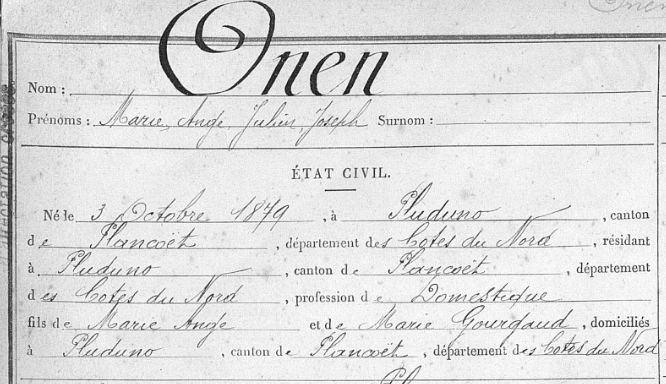
\includegraphics[width=1.0\textwidth]{Identification_EtatCivil_2.PNG}
\caption{\label{fig:id_etatcivil}Identification et \'Etat Civil}
\end{figure}
	    
    On trouve ensuite trois cadres les uns au dessus des autres (figure \ref{fig:classe_signalement}). Le premier correspond au \textit{Num\'ero Matricule de Recrutement}, c'est \`a dire le num\'ero attribu\'e \`a l'individu lors de son recrutement ou engagement (ici le num\'ero 6). Vient ensuite la \textit{Classe de Mobilisation}, qui correspond \`a l'ann\'ee d'engagement. La plupart du temps, c'est l'ann\'ee des vingt ans de l'individu, date \`a laquelle chaque homme apte au service est recrut\'e. Dans ce cas, il arrive que la case ne soit pas renseign\'ee. Cependant, on peut observer des exceptions, notamment dans le cas des engag\'es volontaires, qui s'enr\^olent parfois plus t\^ot. Enfin, un cadre nomm\'e signalement contient le \textit{Signalement}, c'est \`a dire la description physique de l'engag\'e. Plut\^ot qu'un portrait exhaustif, c'est une liste d'attributs : couleur des yeux et cheveux, taille, forme de la bouche du menton ou encore du nez.
    
\begin{figure}[H]
\centering
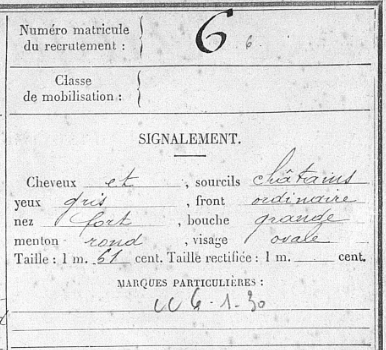
\includegraphics[width=0.7\textwidth]{Classe_Signalement_2.PNG}
\caption{\label{fig:classe_signalement}Num\'ero de matricule, Classe et Signalement}
\end{figure}

    Le plus grand cadre (figure \ref{fig:detailsservice}) est celui qui contient tous les d\'etails sur les activit\'es militaires de l'individu. On y trouve notamment les campagnes auxquelles il a particip\'e, ainsi que les \'eventuelles blessures ou distinctions qu'il a re\c{c}ues. Enfin, si l'individu est d\'ec\'ed\'e ou a disparu durant son service, l'\'ev\`enement est indiqu\'e et dat\'e dans ce cadre.
    
\begin{figure}[H]
\centering
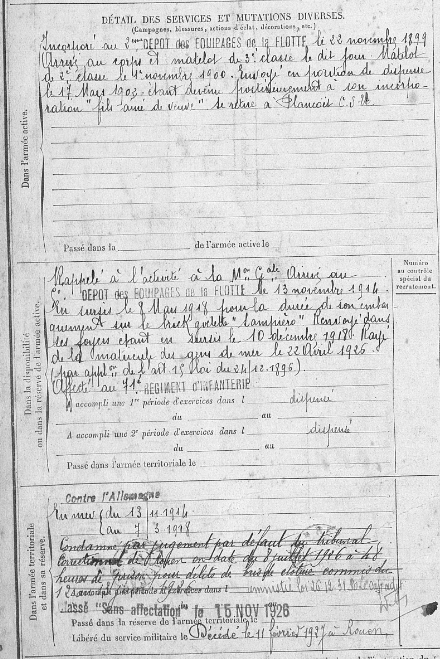
\includegraphics[width=0.9\textwidth]{DetailsService_2.PNG}
\caption{\label{fig:detailsservice}D\'etails des services}
\end{figure}
     
    Les diff\'erents bataillons auxquels l'individu a \'et\'e affect\'e sont contenus dans un autre cadre (figure \ref{fig:affectations}). Ils sont divis\'es en trois cat\'egories, qui correspondent aux trois corps d'arm\'ees de l'\'epoque : l'Arm\'ee Active, la R\'eserve, et l'Arm\'ee Territoriale.
   
\begin{figure}[H]
\centering
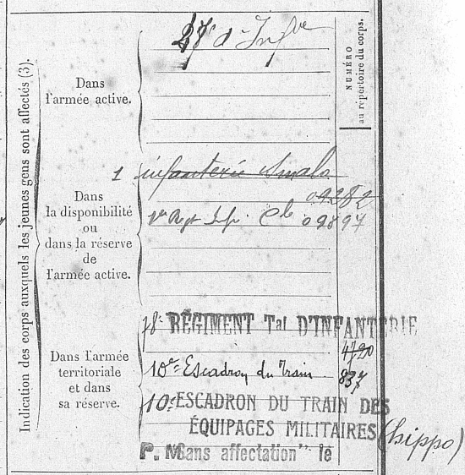
\includegraphics[width=0.6\textwidth]{Affectations_2.PNG}
\caption{\label{fig:affectations}Affectations}
\end{figure}
	
    Enfin, un dernier cadre nomm\'e \textit{Localit\'es Successives Habit\'ees} recense les diff\'erents domiciles de l'individu, afin d'\^etre toujours en mesure de le trouver s'il est appel\'e. M\^eme si ce cadre ne semble pas aussi int\'eressant que les pr\'ec\'edents dans le contexte du centenaire de la Premi\`ere Guere Mondiale, les Archives ont souhait\'e qu'une place lui soit r\'eserv\'ee. En effet, gr\^ace \`a ces donn\'ees, on s'\'eloigne du domaine purement militaire, et on acquiert plut\^ot une vue d'ensemble sur l'individu.
\\
    
\begin{figure}[H]
\centering
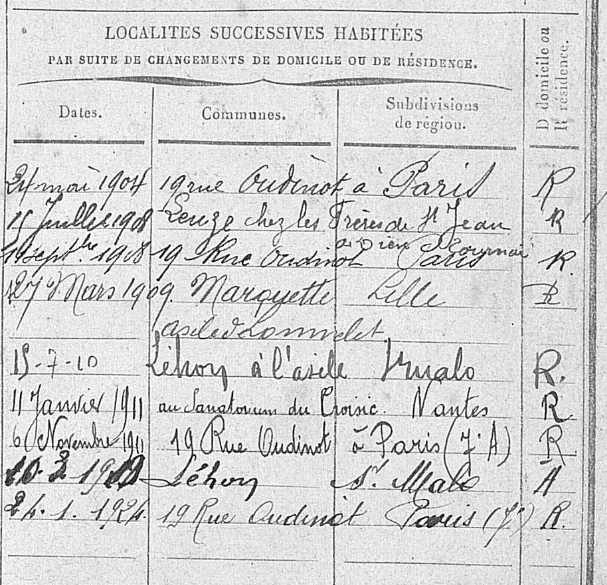
\includegraphics[width=0.6\textwidth]{Domiciles_2.PNG}
\caption{\label{fig:domiciles}Localit\'es Successives Habit\'ees}
\end{figure}
    
    M\^eme si le RMM est en th\'eorie parfaitement d\'ecoup\'e en parties qui contiennent chacunes des donn\'ees sp\'ecifiques, il ne faut pas oublier que ces documents ont \'et\'e renseign\'es par des mains humaines. Ainsi, si certains champs sont g\'en\'eralement compl\'et\'es comme ils devraient l'\^etre, comme l'\'Etat Civil ou le signalement, il arrive que d'autres contiennent des informations qui devraient se trouver ailleurs. Par exemple, il est courant de trouver les diff\'erentes affectations d'un militaire dans le cadre des campagnes, ou encore les mentions de blessures ou d\'ecorations dans les \textit{Localit\'es Successives Habit\'ees}. Du point de vue de notre projet, ces erreurs vont nous obliger \`a proposer un syst\`eme d'annotations tr\`es souple.
\\

	Pour finir, ces documents poss\`edent une autre particularit\'e. Chaque individu est enregistr\'e sur un unique feuillet du RMM, et toutes les informations le concernant doivent \^etre contenues sur ce document. Parfois, l'espace manque, par exemple dans le cas d'un militaire qui a eu de nombreuses affectations. La solution qui a \'et\'e adopt\'ee est celles des retombes (Figure\ref{fig:retombe}). Ce sont des bandes de papier coll\'ees \`a m\^eme le RMM, et sur lesquelles on note les informations manquantes. Ces retombes sont ensuite pli\'ees, afin de laisser visible le texte se trouvant en dessous. On peut les lire simplement en les d\'epliant. Le probl\`eme est que ces retombes obligent les archives \`a scanner plusieurs exemplaires d'un m\^eme RMM : avec retombes ouvertes, et avec retombes ferm\'ees. Heureusement, ces retombes ne sont pas pr\'esentes sur tous les RMM, mais il arrive parfois qu'un seul RMM poss\`ede plusieurs retombes, ce qui accro\^it encore le nombre de prises de vues de ce document.
    
\begin{figure}[H]
\centering
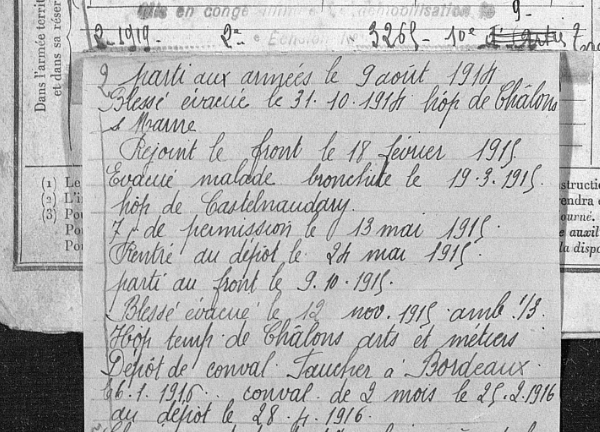
\includegraphics[width=0.8\textwidth]{RetombeOuverte_2.PNG}
\caption{\label{fig:retombe}Retombe Ouverte (d\'epli\'ee)}
\end{figure}
     
     
   

\section{\'Etat de l'art}
\label{sec:etatArt}

\subsection{Outils de gestion des archives}
\label{subsec:outils}

	Les Archives d\'epartementales mettent une partie de leurs documents \`a disposition des visiteurs. Historiquement, ceux-ci devaient se d\'eplacer pour voir ces documents. Aujourd'hui les Archives de chaque d\'epartement proposent de visualiser certains de ces documents en ligne. Pour permettre une navigation plus agr\'eable dans les archives num\'eris\'ees, elles utilisent des logiciels sp\'ecialis\'es.

\subsubsection{Thot}

	Thot est un logiciel m\'etier de gestion et de publication de ressources num\'eris\'ees. Il est d\'evelopp\'e par la soci\'et\'e Sicem et utilis\'e par les archives de plusieurs d\'epartements fran\c{c}ais dont l'Ille-et-Vilaine \cite{thot}. La figure \ref{fig:thot} illustre cet outil. On y voit une page num\'eris\'ee de table de RMM. On retrouve cette page dans son int\'egralit\'e en annexe \ref{sec:annexe 2}.
Puisque nous travaillons avec les Archives d'Ille-et-Vilaine, nous allons proposer un produit bas\'e sur les m\^emes technologies afin de pouvoir y int\'egrer des services Thot.

\begin{figure}[H]
\centering
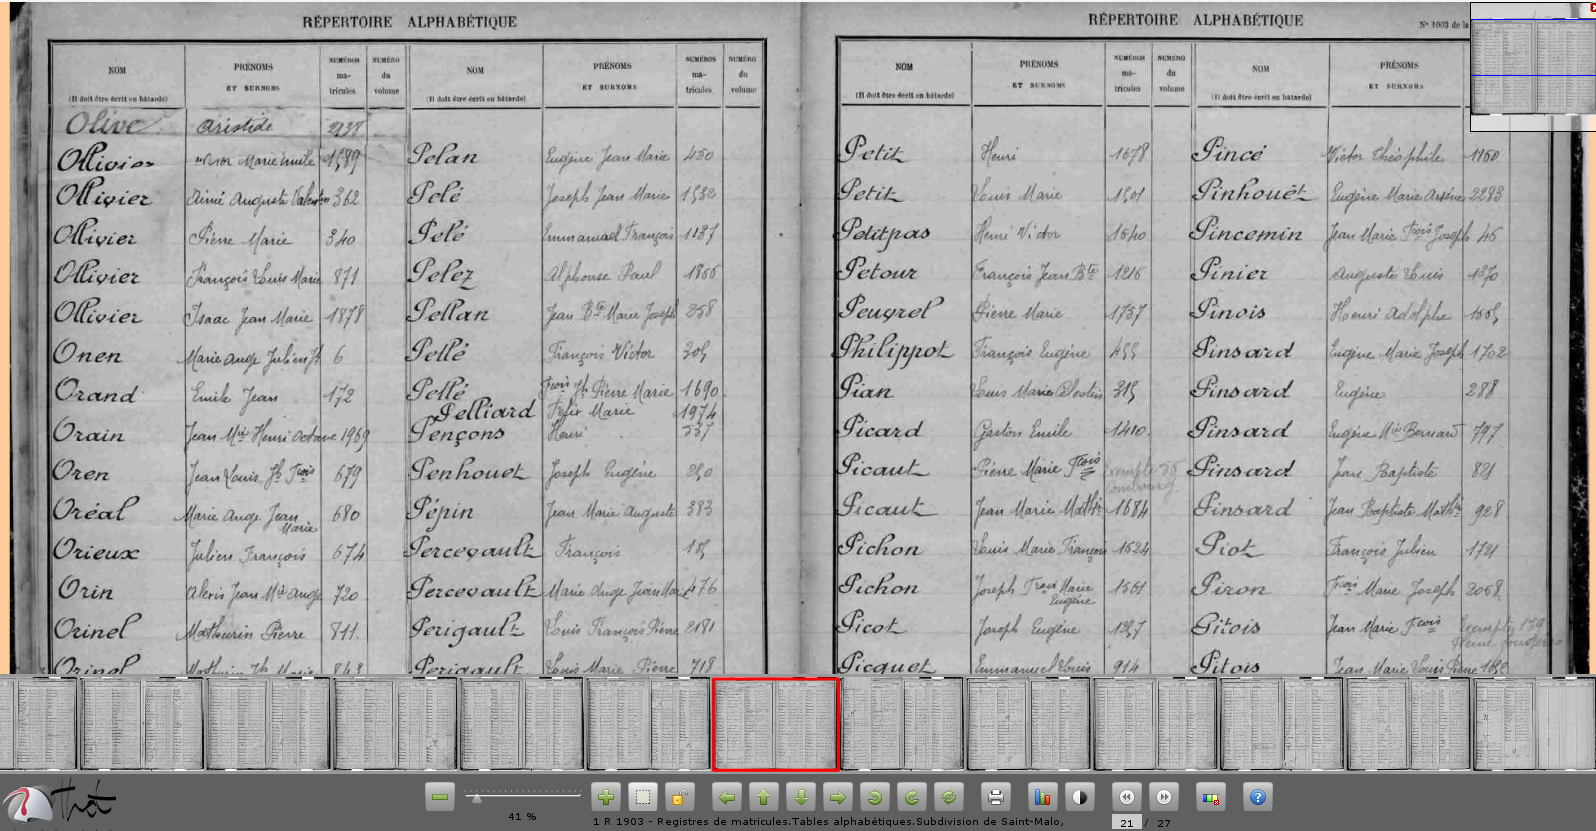
\includegraphics[width=1.0\textwidth]{thot.png}
\caption{\label{fig:thot}Visualisation d'une table de RMM dans Thot.}
\end{figure}

	Les fonctionnalit\'es propos\'ees aux visiteurs lors de l'exploration des documents sont les suivantes :
\begin{itemize}
\item choix du type de document (registres d'\'etat civil, cadastres Napol\'eonien, \ldots),
\item filtrage des r\'esultats par ann\'ee et par commune,
\item outils pour am\'eliorer la visualisation des documents tels que le zoom, la rotation, l'effet n\'egatif, l'impression rapide, la r\'einitialisation des param\`etres.
\end{itemize}
	
	Nous pouvons envisager de reprendre quelques une des ces fonctionnalit\'es dans notre projet afin de rendre plus agr\'eable la navigation au sein des documents.

\subsubsection{Archino\"e}

	Archino\"e est le principal concurrent de Thot parmi les logiciels m\'etier destin\'e \`a la gestion des archives. Comme on le voit dans la figure \ref{fig:archinoe}, leurs interfaces sont similaires. Archino\"e propose notamment des solutions de publication de fonds d'archives, de gestion d'archives et d'archivage \'electronique et est utilis\'e dans un grand nombre de d\'epartements (Vend\'ee, Corr\`eze \cite{archinoe}, Meurthe-et-Moselle, \ldots).

\begin{figure}[H]
\centering
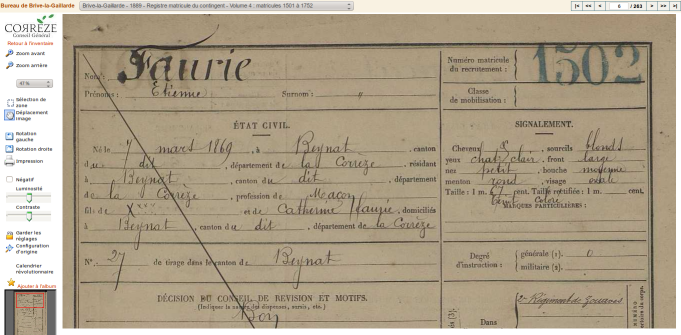
\includegraphics[width=1.0\textwidth]{archinoe.png}
\caption{\label{fig:archinoe}Visualisation d'un RMM dans Archino\"e.}
\end{figure}

	De la m\^eme fa\c{c}on que Thot, Archino\"e propose des fonctionnalit\'es de navigation et de visualisation des documents d'archive.
Leurs fonctions sont similaires, que ce soit pour le d\'eplacement au sein des documents ou pour leur pr\'esentation. Ceci montre l'importance de ces fonctionnalit\'es. Il sera donc important de les implanter dans notre projet.

\subsection{Projets 4INFO}
\label{subsec:projet4info}

\subsubsection{Genovesa}

	Durant l'ann\'ee scolaire 2012-2013, un projet similaire au n\^otre a \'et\'e propos\'e aux \'el\`eves de 4INFO. Les \'etudiants avaient pour objectifs de concevoir un syst\`eme d'annotations et de navigation dans des documents h\'et\'erog\`enes d'archives. Dans un second temps, ils devaient utiliser des informations pivots afin de pouvoir lier les diff\'erents documents se rapportant \`a un individu et ainsi pouvoir collecter un maximum d'informations autour de ce dernier \cite{genovesa}.

	Bien que notre projet ait \'evolu\'e cette ann\'ee, il serait int\'eressant de comprendre le cheminement de leur projet, de r\'eutiliser une partie de leur travail et comprendre comment ils ont surmont\'e leurs difficult\'es. Ceci nous permettra d'optimiser notre temps dans l'objectif de produire un logiciel fini et complet.

	Lors du projet de l'ann\'ee 2012-2013, les \'etudiants ont opt\'e pour un syst\`eme d'annotations g\'en\'erique, capable d'annoter tout type de documents, et utilisant des technologies nouvelles. Ils ont impl\'ement\'e un syst\`eme de navigation au sein des diff\'erents documents et un syst\`eme de visualisation des documents incorporant quelques outils classiques de traitement des images, qu'on retrouve dans Thot et Archino\"e, comme le zoom. Parmi les fonctionnalit\'es importantes de leur syst\`eme, on peut citer le fait qu'une annotation soit associ\'ee \`a un utilisateur. Cependant la modification et la suppression des annotations par l'utilisateur n'ont pas \'et\'e impl\'ement\'ees par manque de temps.
    
\subsubsection{DessofPISee}

Lors de l'ann\'ee scolaire 2011-2012, \'Eric Anquetil de l'\'equipe \bsc{INTUIDOC} avait propos\'e un projet d'annotation de photos entre Microsoft Surface et iPhone. Ce projet avait abouti \`a DessofPiSee \cite{dessofpisee}, une solution permettant le taguage de photos provenant d'un appareil de type iPhone sur une surface plus large, la table tactile Microsoft Surface. 

Deux applications ont \'et\'e d\'evelopp\'ees en parall\`ele. La premi\`ere, sur iPhone, permet de s\'electionner les photos que l'utilisateur veut taguer sur la Surface. Une fois l'iPhone connect\'e \`a la Surface, les photos s\'electionn\'ees sont transf\'er\'ees sur la Surface. Cette application permet \'egalement la visualisation des photos tagu\'ees en retour. La seconde est l'application Microsoft Surface (figure \ref{fig:dessofpisee}). Son objectif est de permettre le parcours et le taguage des photos en offrant une ergonomie optimale.

Lorsque l'utilisateur lance l'application sur Microsoft Surface, les photos import\'ees s'affichent dans une bulle, appel\'ee "bulle initiale". Une autre bulle, contenant les tags, s'affiche \`a l'\'ecran. La bulle des tags va \'evoluer au gr\'e des envies de l'utilisateur. Une mani\`ere simple de taguer une photo est de glisser un tag sur celle-ci.

\begin{figure}[H]
\centering
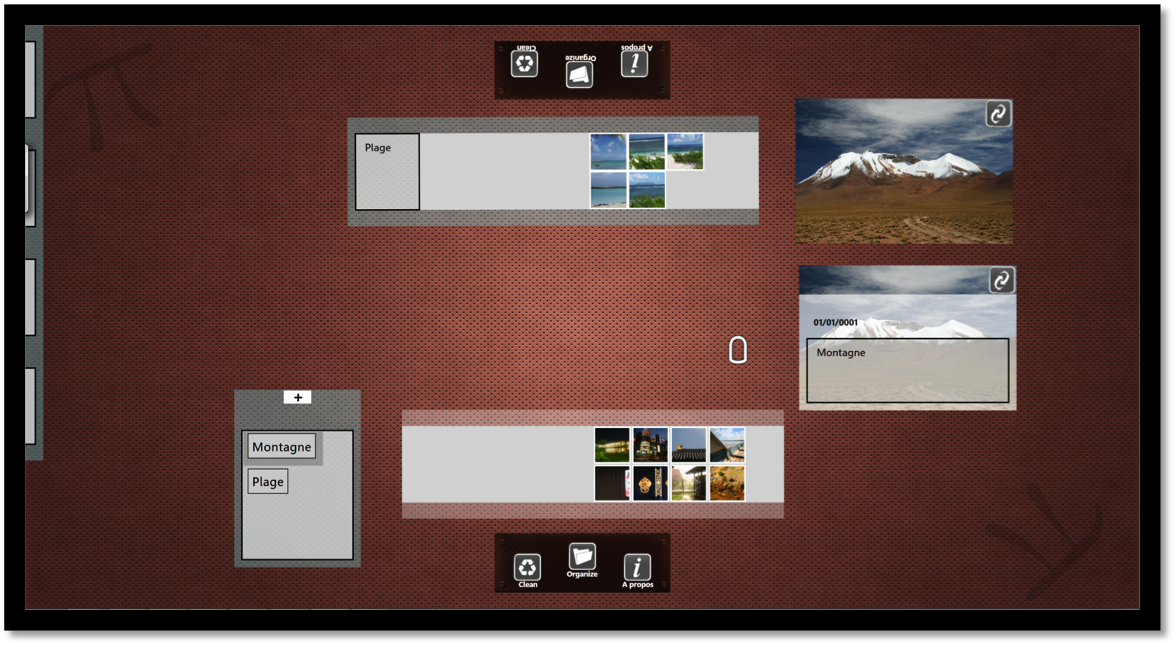
\includegraphics[width=1.0\textwidth]{dessofpisee.png}
\caption{\label{fig:dessofpisee}Application DessofPiSee sur Microsoft Surface}
\end{figure}

Dans le cadre de notre projet, seule l'application sur Microsoft Surface se r\'ev\'ele \^etre int\'eressante sachant que les photos sont la propri\'et\'e des Archives D\'epartementales d'Ille-et-Vilaine.

\subsection{Pr\'ed\'ecoupe des RMM : FormaRead}
\label{subsec:formaread}

	En plus des Archives d'Ille-et-Vilaine, notre projet est encadr\'e par M. Ivan \bsc{Leplumey}, enseignant au d\'epartement informatique de l'\bsc{INSA} de Rennes, mais aussi membre de l'\'equipe \bsc{INTUIDOC}. Cette \'equipe de recherche, sp\'ecialis\'ee dans l'interaction "homme-document", a d\'ej\`a travaill\'e en collaboration avec des Archives d\'epartementales.

	Les registres matricules militaires suivent toujours le m\^eme sch\'ema pour structurer les informations contenues. Or certaines des informations contenues dans ces registres ne peuvent \^etre rendues publique. Par exemple, les informations m\'edicales ne peuvent \^etre divulgu\'ees dans les 120 ans apr\`es la naissance de la personne. C'est pourquoi, \`a la demande des archives de la Mayenne \cite{archive53}, l'\'equipe \bsc{INTUIDOC}, par la personne de Bertrand Co\"uasnon, a propos\'e une solution de d\'ecoupe des registres matricules afin de masquer les parties du document ne pouvant \^etre publi\'ees \cite{formaread}. Cette d\'ecoupe peut s'effectuer sur la majorit\'e des registres, y compris si ces derniers sont ab\^im\'es ou d\'echir\'es.

	Cette solution se r\'ev\`ele tr\`es prometteuse pour notre projet. En effet, nous avons vu dans le chapitre \ref{subsec:rmm} que les RMM pr\'esentent tous une architecture similaire. En exploitant cette architecture, nous pourrions envisager de d\'ecouper ces RMM gr\^ace \`a l'outil de Bertrand Co\"uasnon pour proposer aux utilisateurs des annotations semi-automatiques. Par exemple, nous pourrons rep\'erer qu'une annotation est situ\'ee dans la zone d'\'etat civil gr\^ace \`a l'outil de d\'ecoupage. Nous pourrons alors proposer \`a l'utilisateur des types d'annotations pertinentes, comme la date de naissance ou la profession.

\subsection{Bilan}
\label{subsec:bilanetatart}

	Suite \`a cet \'etat de l'art, nous nous apercevons que nous ne partons pas de rien et que nous avons la possibilit\'e de r\'eutiliser plusieurs outils, ou au moins de nous en inspirer. Par  exemple, nous pouvons repartir du syst\`eme de navigation et de visualisation des documents du projet de l'ann\'ee pr\'ec\'edente, auquel nous ajouterons les outils pr\'esents dans les logiciels Thot et Archino\"e. Outre la navigation et la visualisation des documents, nous devrons r\'eutiliser le projet DessofPiSee pour la visualisation des annotations et le logiciel de pr\'ed\'ecoupe des registres afin de faciliter la gestion des annotations par les utilisateurs.

	En revanche, avec l'approche des comm\'emorations de la Premi\`ere Guerre Mondiale, nous nous focaliserons sur les registres matricules. Il n'est donc pas n\'ecessaire de reprendre un syst\`eme d'annotations g\'en\'eriques tel que pouvait l'\^etre celui propos\'e par les \'etudiants de l'ann\'ee pass\'ee. De plus, les informations pivots ne seront plus utilis\'ees dans le but de faire correspondre les diff\'erents documents mais elles permettront d'effectuer des statistiques sur les profils des personnes ayant particip\'e \`a la Premi\`ere Guerre mondiale.

\section{Sp\'ecifications}
\label{sec:spec}

\subsection{Architecture g\'en\'erale}
\label{subsec:archigenerale}

\begin{figure}[H]
\centering
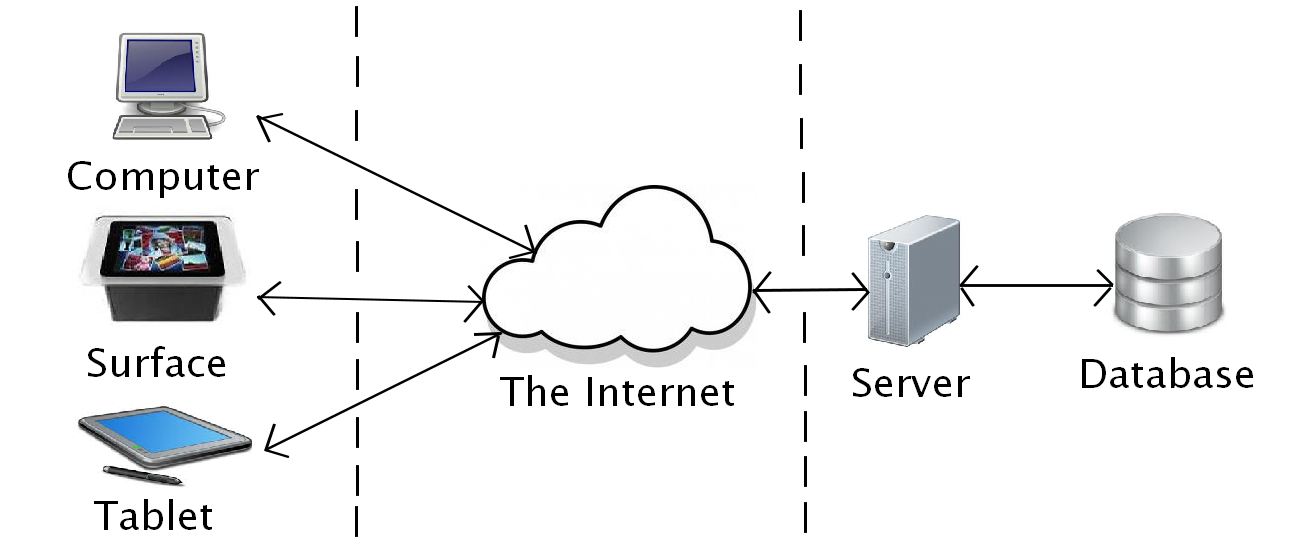
\includegraphics[width=\textwidth]{Specifications_schema_architecture_client_serveur.png}
\caption{\label{fig:architecture}Sch\'ema g\'en\'eral de l'architecture.}
\end{figure}

	L'application fonctionnera dans un environnement client-serveur permettant un mode de communication \`a travers un r\'eseau, ici internet, comme repr\'esent\'ee sur la figure \ref{fig:architecture}. Le logiciel client peut \^etre install\'e sur diff\'erentes machines clientes : table et tablette tactile ou ordinateur. Celui-ci envoie des requ\^etes au serveur \`a travers internet, qui fonctionne comme un r\'eseau \`a \'echelle mondiale. Le serveur attend les requ\^etes, interroge sa base de donn\'ees et envoie la r\'eponse aux clients. Il est n\'ecessaire d'avoir deux types de logiciels pour une m\^eme application : le logiciel client et le logiciel serveur.\\
    
     Pour le moment le choix du support n'est pas d\'efinitif car nous ne sommes pas certains d'avoir acc\`es \`a une table ou tablette tactile. Cependant, nous commencerons \`a d\'evelopper pour une table tactile Microsoft PixelSense. Si toutefois le mat\'eriel nous permettant nos d\'eveloppements ne peut nous \^etre fourni nous reverrons ces sp\'ecifications afin de les adapter \`a un mode PC.
    
\subsection{Sp\'ecifications fonctionnelles}
\label{subsec:fonctionnelles}

	Le principal objectif de l'application est d'annoter des registres matricules dans le but de faciliter une recherche et une lecture de ces documents. L'annotation devra rester propri\'etaire \`a l'auteur. Cependant, elle sera visible par n'importe quel autre utilisateur. Aussi, l'application permettra une navigation et une annotation rapide dans ces images de registres matricules. Elle offrira donc un panel d'outils et de raccourcis dans le but d'am\'eliorer l'efficacit\'e de l'utilisateur.\\
    
	La premi\`ere \'etape est de r\'ealiser un logiciel fonctionnel. Etant donn\'e le temps imparti pour le projet et la multitude de fonctionnalit\'es que nous pourrions impl\'ementer, nous allons prioriser les fonctionnalit\'es afin d'avoir \`a la fin un projet fonctionnel et r\'epondant aux plus grands besoins. Nous verrons si le planning nous permet de d\'evelopper les fonctions moins prioritaires. Nous rentrerons plus dans les d\'etails lors de la phase de conception. Les sous-parties suivantes d\'ecrivent les diff\'erentes m\'ethodes que doit poss\'eder le logiciel tel que peut le d\'ecouvrir un utilisateur. Les fonctionnalit\'es ne sont pas ordonn\'ees en fonction de leur priorit\'e. 
    
\subsubsection{Inscription}


	L'application \'etant multi-utilisateur, celle-ci doit autoriser l'adh\'esion de plusieurs membres. Plusieurs informations seront demand\'ees \`a l'utilisateur afin qu'il puisse s'identifier par la suite : un couple login / mot de passe ainsi que son e-mail utilisateur (liste non exhaustive).\\

	Ces donn\'ees seront stock\'ees sur une base de donn\'ees priv\'ee et en aucun cas les informations de chaque utilisateur ne seront distribu\'ees ou utilis\'ees \`a mauvais escient. \\
    
    Il sera par la suite possible, pour chaque utilisateur, de modifier son mot de passe.\\

	Le login de l'utilisateur permettra de tracer son utilisation sur l'application, par exemple s'il laisse une annotation, un avis. Son email permettra un niveau de s\'ecurit\'e sup\'erieur s'il oublie son mot de passe.
    
\subsubsection{Connexion}

	Deux niveaux d'accessibilit\'es seront permis sur l'application. Un utilisateur non identifi\'e pourra tout de m\^eme consulter les images des registres matricules ainsi que les annotations de chaque utilisateur. Cependant, il ne pourra pas acc\'eder \`a l'\'edition d'annotation et proposer des avis. 
Un utilisateur identifi\'e pourra quant \`a lui, \'editer ses annotations, g\'erer son profil et proposer son avis ou voter.
Pour s'identifier, l'usager devra indiquer son couple login / mot de passe.

\subsubsection{Visualisation des images}

	L'application doit permettre \`a l'utilisateur de naviguer et de visionner les images des registres matricules ainsi que les annotations des diff\'erents utilisateurs. Thot et Archino\"e proposent des outils tr\`es similaires pour faciliter la navigation et la visualisation des images. La figure \ref{fig:modifImage} illustre ces outils. Notre application devra offrir ces m\^emes outils \`a l'utilisateur, parmi lesquels :
\begin{itemize}
\item un zoom, pour permettre \`a l'utilisateur d'agrandir ou de r\'eduire l'image afin de mieux discerner les d\'etails, avec la possibilit\'e de remettre le zoom par d\'efaut,
\item un d\'eplacement de l'image
\item un r\'eglage de la luminosit\'e et du contraste afin de permettre une meilleure lecture de l'image,
\item un film n\'egatif, afin de faire ressortir le texte du support,
\item des rotations, pour lire des textes \'eventuellement \'ecrit de travers.
\end{itemize}

\begin{figure}[H]
\centering
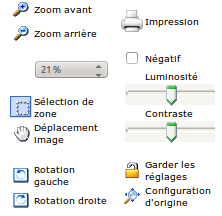
\includegraphics[width=0.5\textwidth]{modification_image_archinoe.png}
\caption{\label{fig:modifImage}Outils de modifications d'image dans Archino\"e ou Thot.}
\end{figure}

	L'utilisateur pourra s\'electionner un dossier contenant toutes les images \`a visualiser, et changer d'image \`a tout moment ou revenir sur les images qu'il a d\'ej\`a vues. Les images seront donc tri\'ees et index\'ees.
Enfin l'utilisateur devra \^etre libre de se d\'eplacer dans l'image si celle-ci est agrandie et donc impossible \`a afficher \`a l'\'ecran dans sa totalit\'e.
\\

	L'utilisateur pourra \'egalement voir les annotations des autres usagers associ\'ees \`a l'image qu'il visionne et importer les annotations rapides d'un de ces usagers pour se les approprier et les modifier par la suite sans impacter les annotations d'origine.\\

	Afin de mettre en valeur les champs les plus importants (c.f. partie \ref{subsec:rmm} RMM), une "fiche d'identit\'e" r\'ecapitulative des annotations importantes sera affich\'ee.  Par exemple, si on recherche un individu avec son nom de famille, on pourra visionner les diff\'erentes fiches d'identit\'es correspondantes.\\

	Beaucoup de pages des registres matricules apparaissent en double ou en triple, voire plus, \`a cause de la pr\'esence de retombes (il est alors n\'ecessaire de num\'eriser le document avec les retombes ouvertes et ferm\'ees pour avoir toutes les informations). L'application rendra possible le regroupement de ces "images doublons" et une navigation "verticale" entre celles-ci.\\

	Enfin, il peut manquer des images dans le dossier d'images import\'ees, auquel cas il serait int\'eressant de le signaler aux Archives d\'epartementales.

\subsubsection{Annotation}

	Le syst\`eme d'\'edition des annotations doit offrir les m\^emes fonctionnalit\'es que le syst\`eme de navigation et de visualisation des images, en offrant en plus un moyen \`a l'utilisateur d'\'editer une annotation. Chaque annotation devra \^etre associ\'ee \`a l'utilisateur qui l'a cr\'e\'ee et \^etre manipulable seulement par lui.\\
    
    Un exemple d'utilisation permet de mieux comprendre pourquoi les prochains points sont utiles. On peut imaginer qu'un utilisateur souhaite survoler et annoter rapidement des images qui d\'efilent, tout en gardant en t\^ete un seul sujet important (par exemple : le nom de famille de la personne), comme un "travail \`a la cha\^ine", c'est-\`a-dire qu'il va mettre dans un favori les diff\'erentes images qui l'int\'eressent pour, dans un deuxi\`eme temps, les annoter. Cependant, il devra \^etre possible de marquer une image qui l'int\'eresse au cours de sa recherche sans qu'elle ait un rapport avec la recherche actuelle, c'est-\`a-dire de l'ajouter \`a un autre favori, pour ensuite y revenir facilement sans interrompre son "travail \`a la cha\^ine" en cours.\\
 
	Ainsi, des cases repr\'esentant des favoris seront disponibles, ou des boutons dans le cas d'un ordinateur. L'utilisateur pourra faire glisser l'image vers cette case pour l'ajouter \`a la cat\'egorie d'image attendue. \\
    
    L'application permettra d'ajouter de nouveaux favoris, par exemple pour la recherche des personnes ayant appartenues \`a la m\^eme famille.\\
    
    L'utilisateur peut ensuite cliquer sur une case pour acc\'eder aux diff\'erentes images contenue dans ce regroupement pour ajouter des annotation \`a chaque image s\'epar\'ement.\\
    
   	Ensuite, l'utilisateur pourra utiliser des cases pour faire des annotations rapides. Des cases d'annotations par d\'efaut peuvent \^etre d\'efinie, par exemple pour signaler qu'un individu \`a \'et\'e "Bless\'e \`a la guerre" ou "M\'edaill\'e".\\
    
	\`A chaque annotation devra \^etre associ\'ee une position afin de faciliter la relecture et la v\'erification.\\

\subsubsection{Recherche}

	L'application doit aussi permettre \`a un utilisateur de rechercher des informations d\'ej\`a annot\'ees par d'autres utilisateurs. L'application pourra int\'egrer des pivots pour r\'eunir les registres entre eux autour d'une information commune (par exemple, conna\^itre tous les soldats ayant particip\'e \`a une bataille).

\subsection{Technique - Technologies}
\label{subsec:techno}

\subsubsection{Table Tactile Microsoft PixelSense}
\label{subsubsec:tabletactile}

\begin{figure}[H]
\centering
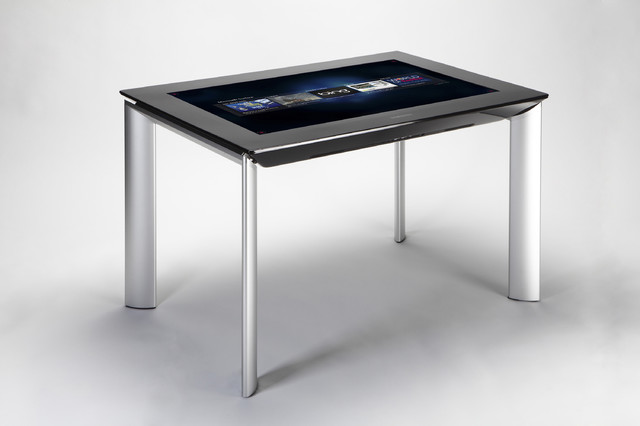
\includegraphics[width=0.7\textwidth]{coffee-tables.png}
\caption{\label{fig:pixelSense}Table Microsoft PixelSense}
\end{figure}
    
La table Microsoft PixelSense, visible dans la figure \ref{fig:pixelSense},  anciennement appel\'ee table Microsoft Surface, est un syst\`eme informatique utilisant la technologie surface computing; elle permet \`a l'utilisateur de manipuler un contenu informatique \`a l'aide d'un \'ecran tactile. Elle a \'et\'e renomm\'ee ainsi pour \'eviter toute confusion avec les tablettes PC Microsoft Surface. Elle se pr\'esente comme une table dont le dessus est constitu\'e d'une surface. Il existe actuellement deux versions. La premi\`ere est dot\'ee d'un affichage tactile multitouch de 30 pouces poss\'edant une r\'esolution de 1024x768 (4:3). Une deuxi\`eme version beaucoup plus perfomante est commercialis\'ee depuis d\'ebut 2012, poss\`edant un \'ecran 40 pouces pour une r\'esolution de 1920x1080 (16:9). Le d\'epartement Informatique de l'INSA de Rennes poss\`ede actuellement les deux versions de cette table. L'INSA souhaite \'egalement commander des \'ecrans tactiles, sur lesquels nous pourrions d\'evelopper notre projet, mais nous ne savons pas s'ils pourront \^etre command\'es \`a temps.\\
    
Si les table tactiles ne sont pas encore destin\'ees au grand public, elles commencent n\'eanmoins \`a bien s'adapter \`a certains milieux professionnels qui n'h\'esitent pas \`a les utiliser. De tr\`es nombreuses applications peuvent se d\'evelopper sur ce type de support. En effet, un \'ecran tactile multitouch poss\`ede plus de possibilit\'es qu'un ordinateur avec un clavier et une souris. D\'evelopper sur ce support serait tr\`es enrichissant. Cependant nous ne savons pas encore si nous aurons acc\`es \`a une table tactile surface. Il est toutefois possible d\'evelopper notre application sur \'emulateur si nous n'avons pas acc\`es \`a l'une de ces tables.

\subsubsection{Base de donn\'ees}
\label{subsubsec:database}

L'application future devra stocker des informations relatives aux utilisateurs, aux annotations ainsi qu'aux images des registres matricules. Il est donc n\'ecessaire d'utiliser une base de donn\'ees afin de pouvoir r\'ealiser ces diff\'erentes possibilit\'es.
\\

Le SGBD (Syst\`eme de Gestion de Base de Donn\'ees) utilis\'e par le logiciel Thot des archives d\'epartementales de Rennes est le syst\`eme Oracle. Oracle utilise une norme de d\'eveloppement PL/SQL et il serait int\'eressant de pr\'evoir une base de donn\'ees \'equivalente et utilisant cette m\^eme norme afin d'ajouter la possibilit\'e aux archives de transf\'erer facilement les bases de donn\'ees. \'Etant donn\'e le co\^ut des licences Oracle, nous allons utiliser un SGBD compatible type MySQL. Oracle propose en plus des fonctionnalit\'es propres \`a leur syst\`eme, et afin d'\'eviter les conflits, notre utilisation de la base de donn\'ees que nous aurons choisie ne devra pas d\'epasser la norme PL/SQL.

\section{Gestion de projet}
\label{sec:gestion_projet}

Gr\^ace \`a nos encadrants, nous avons l'opportunit\'e d'avoir un contact avec la soci\'et\'e ATOS. Karen Fevrier, chef de projet et Scrum Master, va nous \'eclairer pour la partie gestion de projet. Nous nous rendons compte de la chance d'un tel suivi. Elle nous donnera son point de vue sur la r\'edaction des diff\'erents rapports et dossiers ainsi que sur la planification du projet. Son point de vue professionnel nous permettra d'avoir un aper\c{c}u sur la gestion d'un projet.

\subsection{Cycle en V}
\label{subsec:cycleenv}

	Le principe de cycle en V est, en cas de probl\`eme, de limiter les retours aux \'etapes pr\'ec\'edentes. La phase descendante permet de pr\'eparer les attendus des futures \'etapes montantes. La phase montante permet de d\'etecter les d\'efauts en mettant en parall\`ele les \'el\'ements de la phase descendante. C'est pourquoi il est tr\`es important de respecter l'ordre des \'etapes.

\begin{figure}[H]
\centering
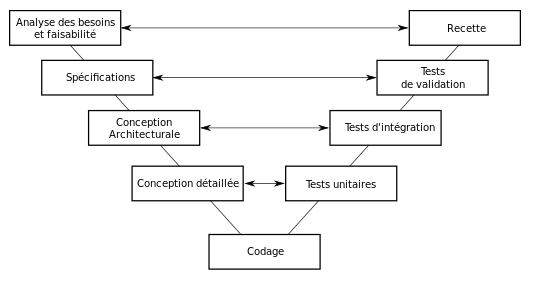
\includegraphics[width=0.5\textwidth]{organisation_cycle_en_v.png}
\caption{\label{fig:cycle_en_v}Sch\'ema du cycle en V.}
\end{figure}

	Il s'agit de la m\'ethode que nous allons adopter pendant le projet, le cycle va nous permettre l'organisation en \'etapes. Cependant, en pratique, il arrive souvent que les \'etapes se chevauchent. Il est tr\`es difficile de s\'eparer les \'etapes de conception du d\'eveloppement par exemple. La conception apporte des solutions pour l'\'ecriture du code, mais lors du d\'eveloppement on se rend compte qu'il est impossible techniquement d'arriver au r\'esultat pr\'evu. Notre planification prendra en compte au maximum cette id\'ee.	

\subsection{Livrables}
\label{subsec:livrables}

	Pendant la dur\'ee du projet plusieurs documents sont \`a produire.
\begin{itemize}
\item \textbf{Rapport de pr\'e-\'etude}, il s'agit d'un rapport pr\'esentant le projet dans sa globalit\'e, il ne faut entrer dans les d\'etails techniques mais seulement d\'ecrire le contexte du projet ainsi que les fonctionnalit\'es. C'est un cahier des charges plus complet.
\begin{itemize}
\item Responsable : Thomas Fran\c{c}ois
\item Version 1 : mercredi 16 octobre
\item Version Finale : jeudi 24 octobre
\end{itemize}
\item \textbf{Dossier de sp\'ecification}, ce document d\'ecrit dans le d\'etail les fonctionnalit\'es et les composants \`a d\'evelopper pour les accomplir.
\begin{itemize}
\item Responsable : Benoit Travers
\item Version 1 : mercredi 20 novembre
\item Version Finale : jeudi 28 novembre
\end{itemize}
\item \textbf{Rapport de planification}, il pr\'esente la planification du projet pour les mois \`a venir. Il est accompagn\'e d'une soutenance.
\begin{itemize}
\item Responsable : Cl\'ement Leboullenger
\item Version 1 : jeudi 12 d\'ecembre
\item Version Finale : mercredi 18 d\'ecembre
\item Soutenance : vendredi 20 d\'ecembre
\end{itemize}
\item \textbf{Dossier de conception}, il d\'ecrit l'architecture interne du logiciel, sa mod\'elisation et l'interfa\c{c}age des diff\'erents modules.
\begin{itemize}
\item Version 1 : vendredi 7 f\'evrier
\item Version Finale : jeudi 13 f\'evrier
\end{itemize}
\item \textbf{Rapport de projet}, il s'agit d'un document pr\'esentant l'ensemble du projet, notamment les probl\`emes rencontr\'es et la mani\`ere par laquelle nous les avons r\'esolu.
\begin{itemize}
\item Version 1 : vendredi 25 avril
\item Version Finale : mercredi 21 mai
\end{itemize}
\end{itemize}

\subsection{Planification}
\label{subsec:retroplanning}
	Une premi\`ere estimation des ressources disponibles est en moyenne 5 heures par semaine (hors r\'eunion) par personne.

	Il est cependant n\'ecessaire de prendre en compte la sp\'ecificit\'e des semaines suivantes, qui pour diverses raisons (e.g. partiels ou vacances) se voient attribuer une ressource de 0 heure par semaine : semaine du lundi 27 novembre, semaines du 23 et 30 d\'ecembre, semaine du 13 janvier, semaine du 10 mars, semaine du 28 avril, semaines du 5 et 12 mai.

	Aussi, des semaines bloqu\'ees ont \'et\'e affect\'ees \`a notre emploi du temps qui nous permettront de nous consacrer enti\`erement \`a notre projet, ces semaines auront une ressource d'environ 5 heures par jour par \'etudiant, soit 25 heures par \'etudiant pour une semaine.

	De plus, nous devons prendre en compte l'absence de Benoit Travers et Thomas Fran\c{c}ois lors du second semestre (mobilit\'e internationale), l'\'equipe sera donc r\'eduite \`a quatre \'etudiants pour le second semestre.

\begin{figure}[H]
\centering
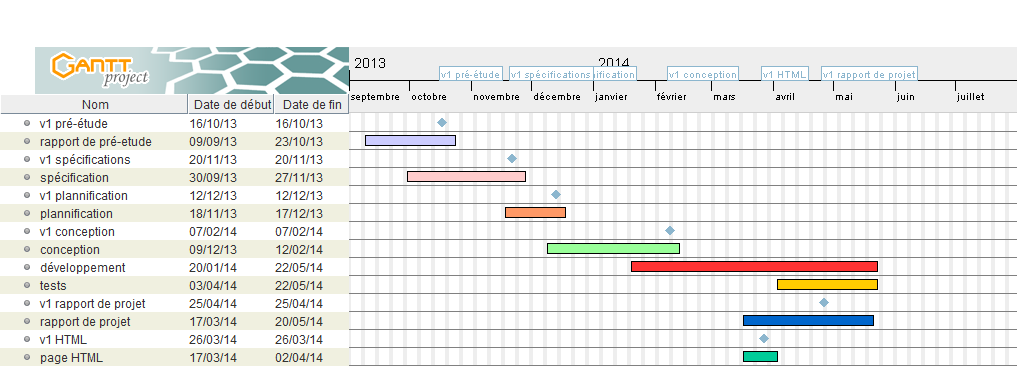
\includegraphics[width=\textwidth]{retro_archive.png}
\caption{\label{fig:retroplanning}R\'etroplanning.}
\end{figure}

\section{Conclusion}
\label{sec:conclusion}

Notre projet a pour objectif d'apporter aux visiteurs des Archives d\'epartementales un outil de navigation, d'annotation et des recherche dans les Registres Matricules Militaires. A l'approche du centenaire de la guerre 14-18, il pourrait devenir pour les Archives un des outils de communication autour des comm\'emorations de la Grande Guerre.

L'application que nous d\'evelopperons proposera des fonctionnalit\'es de recherche et de lecture de RMM, ainsi qu'une fonction d'annotation de ces derniers. Elle permettra ainsi \`a chaque utilisateur des Archives de contribuer \`a une base de connaissance autour de la Premi\`ere Guerre mondiale et de puiser dans cette base pour effectuer ses recherches.

Cette phase de pr\'e-\'etude nous a permis de mieux cerner le projet et ses enjeux. Nous pouvons maintenant commencer la phase de sp\'ecification, durant laquelle nous pr\'eciserons les fonctionnalit\'es de notre application.


\newpage
\section{Glossaire}
\label{sec:glossaire}
\begin{itemize}
\item BMS : bapt\^emes mariages s\'epultures
\item NMD : naissances mariages d\'ec\`es
\item RMM : registres matricules militaires
\item SGBD Oracle : Syst\`eme de gestion de base de donn\'ees Oracle
\end{itemize}


\newpage

\begin{thebibliography}{9}

\bibitem{archive35}
	\emph{Archives d\'epartementales d'Ille-et-Vilaine} [r\'ef. du 21 octobre 2013]. \\
	\url{http://archives.ille-et-vilaine.fr/}
    
\bibitem{thot}
	\emph{Archives et patrimoine d'Ille-et-Vilaine, Thot} [r\'ef. du 21 octobre 2013]. \\
    \url{http://archives-en-ligne.ille-et-vilaine.fr/thot_internet/FrmSommaireFrame.asp}
    
\bibitem{archive53}
	\emph{Archives d\'epartementales de la Mayenne (Utilisant Archino\'e)}  [r\'ef. du 21 octobre 2013]. \\
    \url{http://www.lamayenne.fr/fr/Archives53/Archives-en-ligne}

\bibitem{archinoe}
	\emph{Archives de Corr\`eze (Utilisant Archino\'e)}  [r\'ef. du 21 octobre 2013]. \\
    \url{http://www.archinoe.fr/cg19/registre.php}
    
\bibitem{genovesa}
	Genovesa - INSA Rennes - D\'epartement Informatique - Projet de 4\up{\`eme} ann\'ee - 2012/2013 \\
	Encadrants : Ivan \bsc{Leplumey} - Marie \bsc{Babel} \\
	\'Etudiants : Alexandre \bsc{B\'erard} - Jean \bsc{Guegant} - Vincent \bsc{Guilpain} - Richard \bsc{Lagrange} - Yannick \bsc{Le Pennec} - Gabriel \bsc{Malkas}\\
	\emph{Rapport final - 28 mai 2013}
  
\bibitem{dessofpisee}
	DessofPiSee - INSA Rennes - D\'epartement Informatique - Projet de 4\up{\`eme} ann\'ee - 2011/2012 \\
	Encadrants : Eric \bsc{Anquetil} - Thierry \bsc{Roger} - Pascal \bsc{Fresnay} \\
	\'Etudiants : Reda \bsc{Balkouch} - Ouadie \bsc{Boussaid} - Victor \bsc{Dormagen} - Emmanuel \bsc{Gilles} - Alban \bsc{Granger} - Maxime \bsc{Lelandais} \\
	\emph{Rapport final - 29 mai 2012}

\bibitem{formaread}
    Bertrand \bsc{Co\"uasnon}, Jean \bsc{Camillerapp}, Ivan \bsc{Leplumey}.  \\
	\emph{Access by Content to Handwritten Archive Documents: Generic Document Recognition Method and Platform for Annotations. International Journal on Document Analysis and Recognition, IJDAR, 9(2):223-242, 2007, page 232.}
    
\end{thebibliography}

\appendix


\section{Convention de non-divulgation des images fournies par les Archives}
\label{sec:annexe 3}

\begin{figure}[H]
\centering
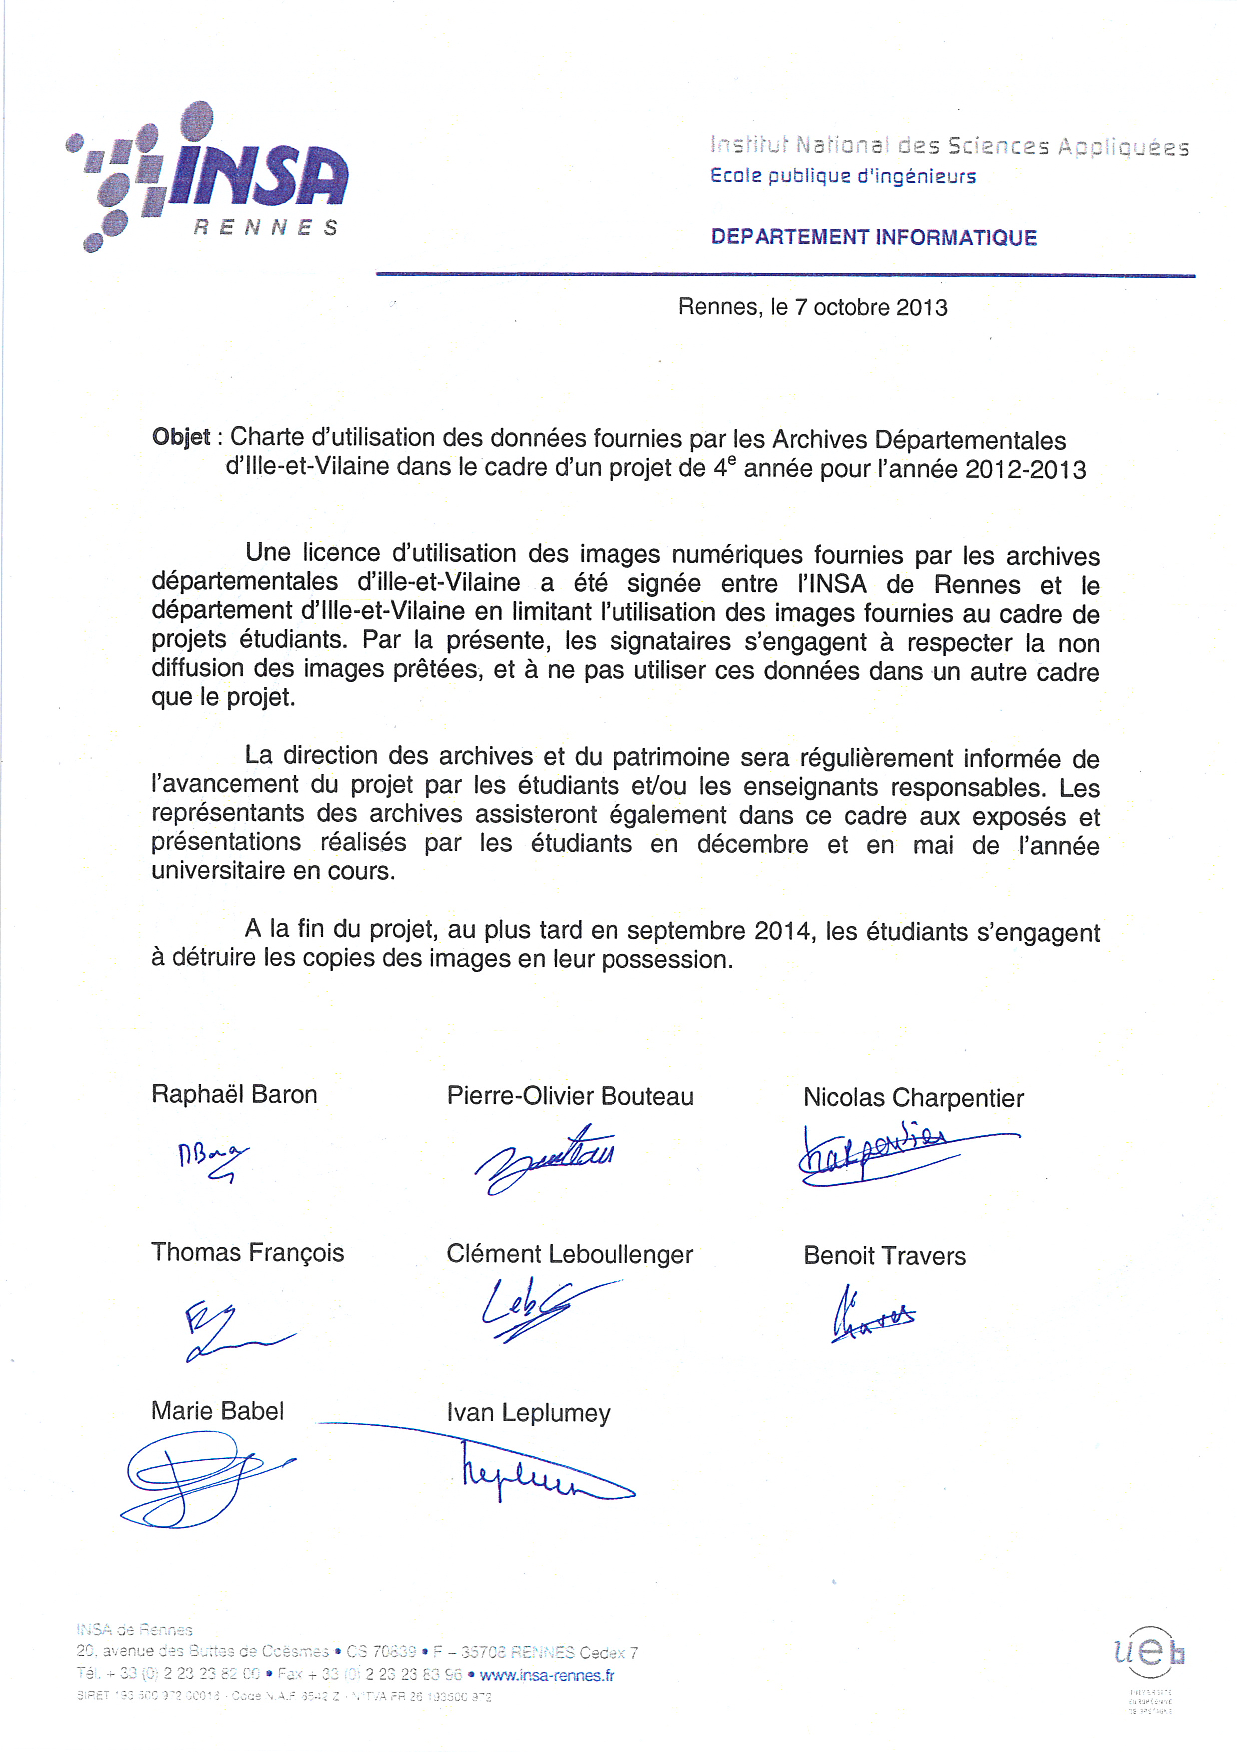
\includegraphics[width=\textwidth]{Convention2013.pdf}
\end{figure}

\section{Vue compl\`ete d'un RMM}
\label{sec:annexe 1}

\begin{figure}[H]
\centering
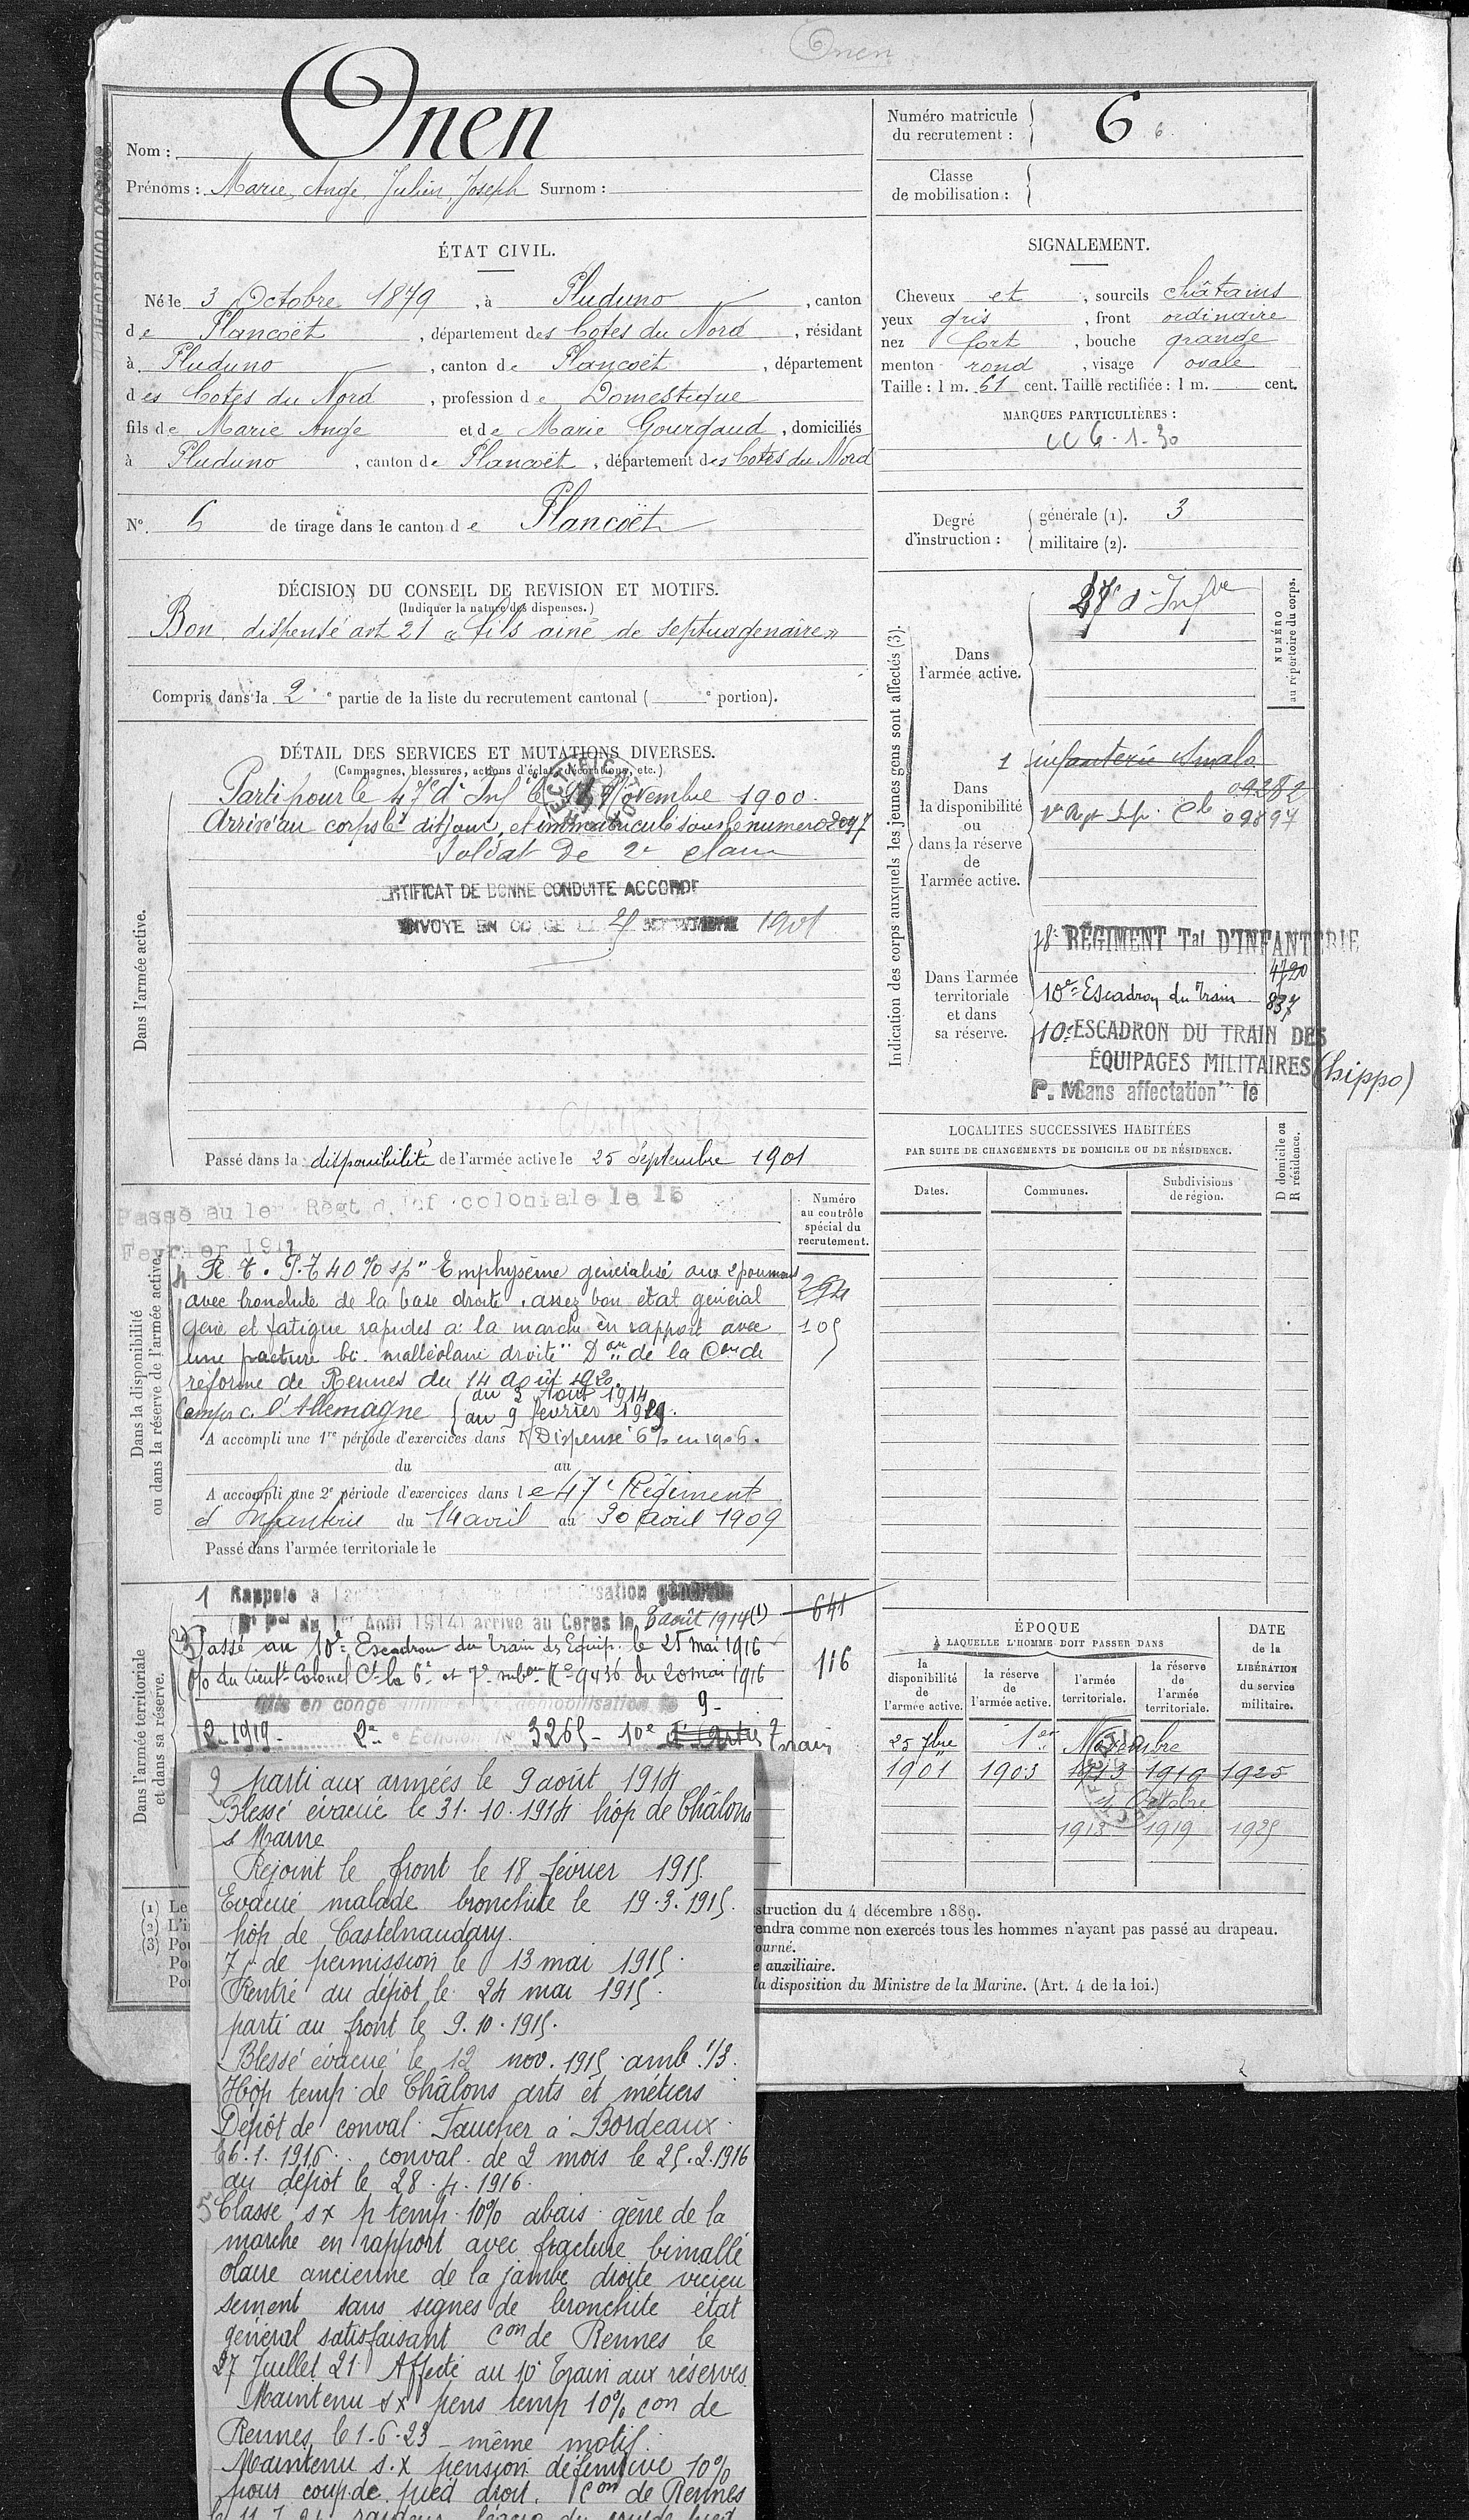
\includegraphics[width=0.95\textwidth]{RMM.JPG}
\end{figure}

\section{Table de RMM - Saint-Malo 1899}
\label{sec:annexe 2}

\begin{figure}[H]
\centering
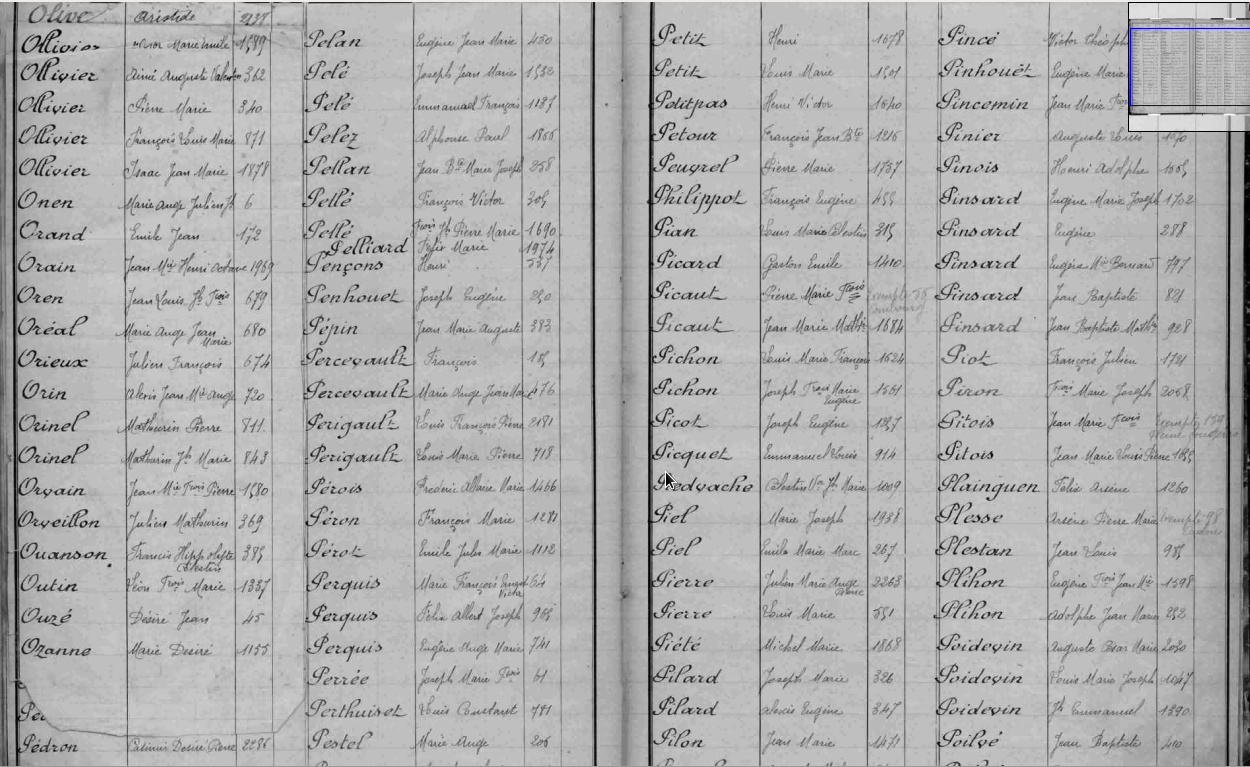
\includegraphics[width=\textwidth]{Table_Onen.png}
\end{figure}

\newpage
\listoffigures


\end{document}